\documentclass[11pt]{article}

\usepackage[scaled]{helvet}
\usepackage[T1]{fontenc}
\renewcommand\familydefault{\sfdefault}

\usepackage[margin=1in]{geometry}

\usepackage[utf8]{inputenc}
\usepackage{amsmath}
\usepackage{algpseudocode}

\usepackage{algorithm}
\usepackage{graphicx}
\usepackage[justification=centering]{caption}

\usepackage{cite}

\algnewcommand\algorithmicforeach{\textbf{parallel for each}}
\algdef{S}[FOR]{ForEach}[1]{\algorithmicforeach\ #1\ \algorithmicdo}

\title{Induced 6-Cycle Counting in Bipartite Graphs}

\begin{document}

\maketitle

\begin{abstract}
Finding subgraphs in a bipartite graph is crucial to understanding its underlying structure.
The smallest non-trivial subgraph in a bipartite graph is a 4-cycle, which is also known as a butterfly.
Shi and Shun recently used the affordances of parallization to develop efficient butterfly counting algorithms.
However, parallel approaches to counting larger cycles is a relatively unexplored area.
In this paper, we propose a parallel algorithm for efficiently counting induced 6-cycles.
\end{abstract}

\section{Introduction}
Many real-world networks are represented by a bipartite graph.
For example, recommendation networks often are represented as a bipartite graph with users on one partition and items on the other \cite{li2013recommendation}.
Finding graph motifs that form the building blocks of these networks can reveal the underlying structure within bipartite graphs.

In unipartite graphs, the smallest cycle is a 3-cycle, which is also known as a triangle.
However, since bipartite graphs contain no odd cycles, triangles do not exist in bipartite graphs.
The smallest cycle in a bipartite graph is a 4-cycle, which is also known as a butterfly.
Butterflies are the smallest building blocks for community structures in bipartite graphs.

\begin{figure}[h]
    \centering
    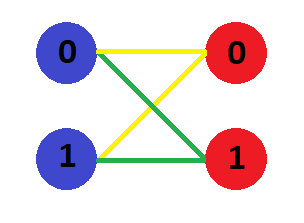
\includegraphics[width=0.25\textwidth]{figures/Butterfly.png}
    \caption{\small This graph depicts a butterfly. Nodes in u are in blue while nodes in v are in red. The butterfly is made of two wedges, which are highlighted in yellow and green.}
    \label{fig:butterfly}
\end{figure}

Counting cycles in bipartite graphs is NP-hard \cite{flum2004parameterized}.
Sequential algorithms for butterfly counting use the concept of combining wedges (2-paths) to count butterflies (see Figure 1) \cite{wang2014rectangle, sanei2018butterfly, chiba1985arboricity}.
When dealing with larger graphs, however, the runtime of sequential algorithms may be problematic.
Adapting sequential algorithms for parallization can significantly reduce the runtime of these algorithms.
Shi and Shun \cite{shi2019parallel} recently designed a parallel butterfly counting algorithm which modified Chiba and Nishizeki's wedge retrieval process \cite{chiba1985arboricity} to enable parallization.

\begin{figure}[h]
    \centering
    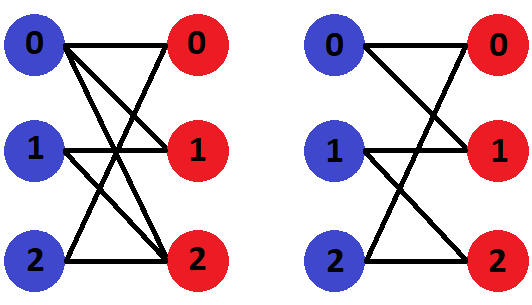
\includegraphics[width=0.25\textwidth]{figures/Induced vs Noninduced.png}
    \caption{\small The graph on the left depicts a non-induced 6-cycle. The graph on the right depicts an induced 6-cycle. Nodes in u are in blue while nodes in v are in red. In the non-induced graph, the removal of the edge from u0 to v2 won't affect the 6-cycle.}
    \label{fig:induced}
\end{figure}

Given the relevance of bipartite graphs in real-world relationships, it is desirable to find larger cycles within these graphs.
Karimi and Banihashemi \cite{karimi2012message} designed a message-passing algorithm for counting cycles of length \textit{g} to \textit{2g-2} in bipartite graphs, where \textit{g} is the girth of the graph.
Dehghan and Banihashemi \cite{dehghan2019counting} proposed an algorithm that uses breadth-first search to count cycles of length \textit{g}  to \textit{g+4} in bipartite graphs.
However, these sequential algorithms have only been tested on small bipartite graphs.
Parallizing algorithms that count larger cycles is extremely valuable due to their increased complexity.
This paper presents a framework for counting induced 6-cycles (see Figure 2) in bipartite graphs which uses the affordances of parallization to maximize efficiency.

\section{Notation}
We work on a simple and undirected bipartite graph \textit{G = (U, V, E)} where \textit{U} is the set of nodes in the left set, \textit{V} is the set of nodes in right set, and \textit{E} is the set of edges.
The neighbors of a node \textit{v} is denoted by \textit{N(v)}.
The ranking of a node \textit{v} is denoted by \textit{R(v)}.
A \textbf{wedge} is a set of three nodes \textit{u1, u2} $\in$ \textit{U} and \textit{v} $\in$ \textit{V} composed of edges \textit{(u1, v), (u2, v)} $\in$ \textit{E}. 
We call the nodes \textit{u1, u2} \textbf{endpoints} and the node \textit{v} the \textbf{center}.
An \textbf{induced 6-cycle} is a set of six nodes \textit{u1, u2, u3} $\in$ \textit{U} and \textit{v1, v2, v3} $\in$ \textit{V} such that its internal edges exactly form a cycle.

\section{Algorithm}

We introduce a parallel algorithm for counting induced 6-cycles in bipartite graphs.
Our algorithm extends the parallel wedge retrieval algorithm proposed by Shi and Shun \cite{shi2019parallel}.

\begin{algorithm}[H]
\caption{Preprocessing(\textit{G})}
\hspace*{\algorithmicindent} \textbf{Input:} \textit{G}: graph \\
\hspace*{\algorithmicindent} \textbf{Output:} \textit{R}: ranking of nodes
\begin{algorithmic}[1]
    \State $X \gets Sort(U \cup V)$ \Comment sort vertices in decreasing order of degree
    \State Let $x$'s rank $R(x)$ be its index in $X$
    \ForEach {$x \in X$}
        \State $N(x) \gets Sort({y | (x, y) \in E})$ \Comment sort neighbors by decreasing order of rank
    \EndFor
    \State return $R$
\end{algorithmic}
\end{algorithm}

We give a preprocessing algorithm (Algorithm 1) that takes as input a bipartite graph and returns a ranking of nodes in decreasing order of degree.
Preprocessing also sorts neighbors by decreasing order of rank.
Shi and Shun \cite{shi2019parallel} proved that using approximate degree ordering, complement degeneracy ordering, and approximate complement degeneracy ordering also gives work-efficient bounds.
By establishing an ordering of nodes, we can avoid traversing the same induced 6-cycle twice.

\begin{algorithm}[H]
\caption{GetWedges(\textit{G}, \textit{R})}
\hspace*{\algorithmicindent} \textbf{Input:} \textit{G}: graph, \textit{R}: ranking of nodes \\
\hspace*{\algorithmicindent} \textbf{Output:} \textit{W}: list of wedges
\begin{algorithmic}[1]
    \State initialize $W$
    \ForEach {$u1 \in U \cup V$}
        \ForEach {$v \in N(u1)$}
            \If{$R(v) > R(u1)$}
                \ForEach {$u2 \in N(v)$}
                    \If{$R(u2) > R(u1)$}
                        \State $W((u1, u2, v))$
                    \Else
                        \State break
                    \EndIf
                \EndFor
            \Else
                \State break
            \EndIf
        \EndFor
    \EndFor
    \State return $W$
\end{algorithmic}
\end{algorithm}

We define a wedge retrieval algorithm, GetWedges (Algorithm 2), that takes as input a preprocessed graph and its ranking \textit{R}.
We use \textit{W} to denote a parallel unordered container such that \textit{W(x)} stores \textit{x} in the container.
GetWedges is based off of Shi and Shun \cite{shi2019parallel} wedge retrieval algorithm which enables the parallel processing of wedges.
For all nodes \textit{u1} in \textit{G}, the algorithm retrieves all wedges with endpoints \textit{u1, u2} and center \textit{v} such that \textit{u2} and \textit{v} both have rank greater than \textit{u1}.

\begin{algorithm}[H]
\caption{BFSCount(\textit{G}, \textit{R}, \textit{w})}
\hspace*{\algorithmicindent} \textbf{Input:} \textit{G}: graph, \textit{R}: ranking of nodes, and \textit{w}: wedge \\
\hspace*{\algorithmicindent} \textbf{Output:} \textit{c}: count of induced 6-cycles
\begin{algorithmic}[1]
    \State $c \gets 0$
    \State $u1, u2, v \gets w$
    \State For any node $u \in G, d(u)$ = $\infty$
    \State $d(u2) \gets 0$
    \State Let $Q \gets$ queue
    \State $Q.enqueue(u2)$
    \While {$Q$ is not empty}
        \State $x = Q.dequeue$
        \ForEach {$y \in N(x)$}
            \If{$d(y) = \infty$}
                \State $d(y) \gets d(x) + 1$
                \If{$d(y) = 1$}
                    \If{$R(y) > R(v)$ and $y \not\in N(u1)$}
                        \State $Q.enqueue(y)$
                    \EndIf
                \ElsIf{$d(y) = 2$}
                    \If{$y \not\in N(v)$}
                        \State $Q.enqueue(y)$
                    \EndIf
                \ElsIf{$d(y) = 3$}
                    \If{$R(y) > R(v)$ and $y \not\in N(u2)$}
                        \State $Q.enqueue(y)$
                    \EndIf
                \Else
                    \If{$y = u1$}
                        \State $c \gets c + 1$
                        \State $d(y) \gets \infty$
                    \EndIf
                \EndIf
            \EndIf
        \EndFor
    \EndWhile
    \State return $c$
\end{algorithmic}
\end{algorithm}

BFSCount (Algorithm 3) is a modified version of the traditional breadth-first search algorithm.
The algorithm takes as input a wedge \textit{w = (u1, u2, v)} and returns the number of induced 6-cycles with nodes \textit{u1, u2, u3} $\in$ \textit{U} and \textit{v, v2, v3} $\in$ \textit{V} such that \textit{v2} and \textit{v3} both have rank greater than \textit{v}.

\begin{algorithm}[H]
\caption{Par6CycleCount(\textit{G})}
\hspace*{\algorithmicindent} \textbf{Input:} \textit{G}: graph \\
\hspace*{\algorithmicindent} \textbf{Output:} \textit{c}: count of induced 6-cycles
\begin{algorithmic}[1]
    \State $R \gets Preprocessing(G)$
    \State $W \gets GetWedges(G, R)$
    \State $c \gets $0
    \ForEach {$w \in W$}
        \State $c \gets c + BFSCount(G, R, w)$
    \EndFor
    \State return $c$
\end{algorithmic}
\end{algorithm}

We now describe the full induced 6-cycle counting algorithm, which is given as Par6CycleCount in algorithm 4.
Given a bipartite graph G, this algorithm applies G to the preprocessing and wedge retrieval algorithms described in algorithms 1 and 2, respectively.
The summation of applying the modified BFS algorithm in algorithm 3 to each retrieved wedge is then returned as the total induced 6-cycle count.

The code used for this report is available at https://github.com/Deerjason/par6cycle.
Parallization is achieved through the use of Intel Threading Building Blocks due to its multicore capabilities.
Currently, parallel butterfly counting is implemented in the develop branch in butterflyCount.cpp.

\bibliography{report.bib}{}
\bibliographystyle{plain}

\end{document}
